%\documentclass{beamer}
%\usetheme{Pittsburgh} 
\documentclass{scrartcl}

\usepackage[utf8]{inputenc}
\usepackage{default}
\usepackage[procnames]{listings}
\usepackage{graphicx}
%\usepackage[toc,page]{appendix}
\usepackage{caption}
\usepackage{hyperref}
\usepackage{color}
\usepackage{mathrsfs}


%Bibliogrpahy?
\usepackage{bibentry}
%\nobibliography*
%\bibentry{ }


\begin{document}

\title{Reading Summary}
\subtitle{}
\author{
  Quignon, Christophe \\
  %Familyname, Name
} 
\date{\today}


\maketitle

\section{Read Chapter 1 from Haykin’s book; summarize or sketch your insights in mind-map or an outline or a summary.}

\begin{figure}
 \center
 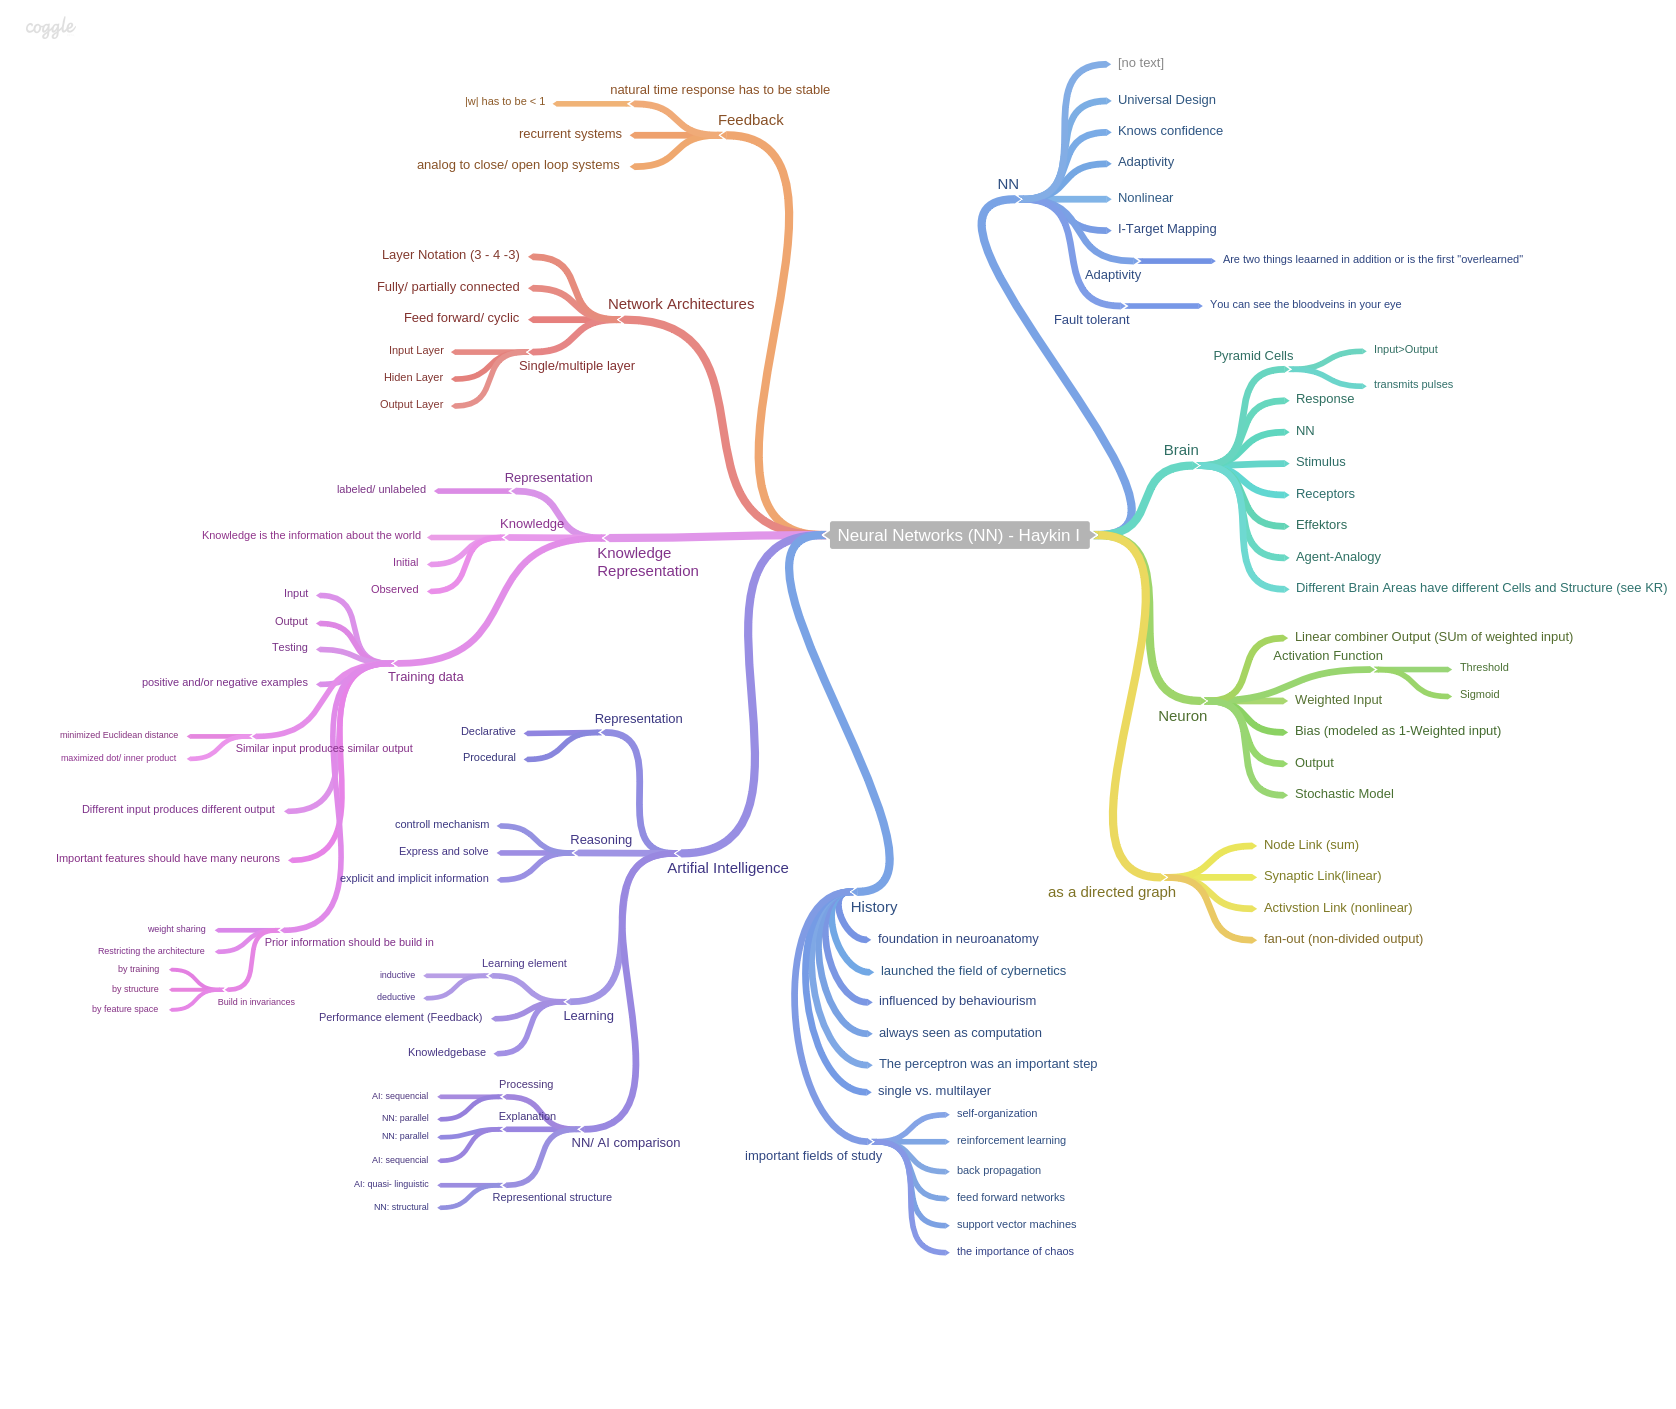
\includegraphics[width= \textwidth]{mindmap.png}
 \caption{Mindmap of chapter one}
 \label{fig:mindmap}
\end{figure}

See figure~\ref{fig:mindmap}.


\section{Read chapter 2 from Haykin’s book until 2.13 (leaving out Statistical learning theory to
end of chapter) and summarize or sketch your insights in mind-map or an outline or a
summary.
}
\begin{enumerate}
\item Introduction
	\begin{itemize}
	\item Learning from the environment and improving performance are key properties of a NN.
	\item The learning process has three major steps:
		\begin{itemize}
		\item stimulation of the NN
		\item change of the NN
		\item new respond of the NN
		\end{itemize}
	\end{itemize}
\item Error Correction Learning
	\begin{itemize}
	\item The error is defines ad the desired output - the actual output
	\item We want to minimize this error by adding costs to it. 
	\item This is called delta rule or Widrow-off rule.
	\item The adjustment of a neuron is proportional to the neurons input and error.
	\item To minimize the error, it must be observable.
	\item This proportion is denoted in the learning-rate parameter $\eta$ (eta)
	\item The tuning of $\eta$ is critical for a NN.
	\end{itemize}
\item Memory Based Learning
	\begin{itemize}
	\item Memory based learning involves:
		\begin{itemize}
		\item A criterion to define the local neighborhood to test against.
		\item A learning rule to be applied to the neighborhood
		\end{itemize}
		
	\item under certain circumstances (infinite sample size, identical and independent distribution), the error of the nearest neighbor is proven to be bounded to twice the bayesian probability of the error.
	\item The number of neighbors compared may vary.
	\item Outliers may be discarded.
	\end{itemize}
	
\item HEBBIAN Learning
	\begin{itemize}
	\item There are two major steps in hebbs learning:
		\begin{itemize}
			\item What fires together, wires together (enhancement)
			\item Neurons that are activated asynchronous, weaken their synapses. (depression)
		\end{itemize}
		\item From that we deduce four basic observations:
			\begin{itemize}
			\item Synaptic strengthening is time dependent
			\item It is dependent on the location of the neurons
			\item It is an interactive mechanism, because it takes neurons in front and after the the activated neurons in consideration
			\item It is a correlated mechanism, because the strengthening involves two. 
			\end{itemize}
		\item From Hebbian synapses, non-hebian and anti-hebian synapses are defined.
		\item Hebb's hypothesis may be varied with the learnig rate $\eta$
		\item It may furthe be improved by the covariance hypothesis with takes previous and following synaptic signals into consideration (averaged).
		\item This allow convergence and predicion of potentiation or depression
		\item The hippocampus is formed by hebbian learning. 
	\end{itemize}
	
\item Competitive learning
	\begin{itemize}
	\item In competitive learning, only one neuron is active at any time. The neurons compete to become this one active neuron.
	\item There are three basic elements to competitive learning:
		\begin{itemize}
		\item Weights are randomly distributed
		\item There is a limit to the strength of a neuron
		\item A mechanism to permit neuron activation, so only one neuron is active (winner takes it all)
		\end{itemize}
	\item To become a winner in a competitive learning NN, neurons become specialists: feature detectors.
	\item In a competitive learning NN, the neurons of one layer may be connected to inhibit their firing. (lateral inhibition)
	\item A neuron learns by shifting weights from inactive to active inputs
	\item A good example of competitive learning is clustering
	\end{itemize}
	
\item Boltzmann learning
	\begin{itemize}
	\item Boltzmann learning is inspired by statistical mechanics.
	\item The neurons activation is binary
	\item The network is defined by an energy function
	\item The activation of the neurons flip at random
	\item This flip changes the energy function and will end in a thermal equilibrium.
	\item The Boltzmann NN has two kinds of neurons:
		\begin{itemize}
		\item visible neurons which are the interface to the environment (may be fixed)
		\item hidden neurons who operate freely
		\end{itemize}
	\end{itemize}
	
\item Credit assignment problem
	\begin{itemize}
	\item The credit assignment problem is the task to divide the reward of a successful to the single components. (Same for unsuccessful)
	\item The problem is dependent on the time of the success (temporal credit-assignment)
	\item It is also concerned with the weighting of the success to the internal structure (structural credit assignment problem)
	\end{itemize}
	
\item Learning with a teacher
	\begin{itemize}
	\item A teacher already learned the desired output
	\item The difference between the teacher output (desired) and the output of the learning system is fed back
	\item The teacher is the optimum to reach
 	\end{itemize}
 	
\item Learning without teacher
	\begin{itemize}
	\item Without a teacher it is hard to find the error.
	\item A critic, who acknowledges good moves, is introduced
	\item In reinforcement learning the system can learn how to optimally approach a goal by delaying the reinforcement
	\item This includes the temporal credit assignment problem
	\item Reinforcement learning is closely related to dynamic programming.
	\item Unsupervised learning was neither a teacher nor a critic
	\item Unsupervised learning uses competitive neurons
	\end{itemize}
	
\item Learning tasks
	\begin{itemize}
	\item Pattern association may happen autoassociative (comparison to stored goal) or heteroassociative (input output pairs)
	\item In pattern recognition, inputs are put into classes by similarity
	\item Pattern recognition is split into feature extraction and classification
	\item Function approximation can be done with system identification  (memoryless MIMO) or with inverse system 
	\item Control can also efficiently be learned with a NN
	\item NN control can handle nonlinear noise and develop longtime plans
	\item Control learning may happen indirect with the systems in and output or direct with the signs of the partial derivatives
	\item Filtering of noise with filters, smoothing or prediction is a common field of NN learning
	\item Beamforming as a subfield of filtering because it copes with cut out beams of information from the environment
	\end{itemize}

\item Memory
	\begin{itemize}
	\item Characteristics:
		\begin{itemize}
		\item distributed
		\item both stimulus and response are stored 
		\item memory is resistant to noise
		\item interactions between patterns are also stored
		\end{itemize}
	\item The memory can be stored in memory matrix which contains the weight of all neuronal connections
	\item One fundamental function of the memory is to recall patterns
	\end{itemize}
	
\item Adaptation
	\begin{itemize}
	\item It is crucial to adapt behaviour with respect to the time
	\item Only non-static environments have a time component to which the NN has to adapt to.
	\item  However, some signals (speech, radar) are stationary over a certain period of time
	\item This pseudostationary property can be exploited (only use change, change monitoring time)
	\end{itemize}
\end{enumerate}


\section{Read chapter 2 from Haykin’s book (2nd edition), starting from section 2.13 to end of
chapter, leaving out section 2.15 (PAC learning). Summarize or sketch your insights in
mind-map or an outline or a summary.
}
\begin{enumerate}
\setcounter{enumi}{12}
\item Statistical Nature of the Learning Process
	\begin{itemize}
	\item For every measurement there is an error $\epsilon$ which we assume to be zero mean and random occurrence.
	\item This error can be modelled with regression.
	\item We can not know the bias, only the variance of an error.
	\item the price for a small bias is a large variance.
	\item the bias can only be minimized by the design of the NN
	\end{itemize}
\item statistical learning theory
	\begin{itemize}
	\item A learning model has three components:
		\begin{itemize}
		\item The Environment (supplying input $x$)
		\item The teacher (supplying desired response $d$)
		\item The learning algorithm (Mapping $x$ to $d$)
		\end{itemize}
	\item There is a loss $L$ or discrepancy between the actual and the desired output
	\item The expected Loss is defined by the risk function $R(w)$
	\item With empirical risk minimization we can minimize the risk with respect to the weights $w$
	\item The VC dimension measures the capacity of the family of classification functions.
	\item the VC dim is a combinatorial concept that is unrelated to geometry
	\item The vc dim of a multilayered feedforward network with a sigmoid activation function is $O(W^{2})$, where $W$ is the number of free parameters.
	\item the training error is the frequency of errors during learning
	\item the generalization error is the frequency of error after training
	\item the generalization error is bound by the guaranteed risk
	\item the guaranteed risk depends on the confidence interval and the training error. 
	\item the guaranteed risk has minimum that can be found by structural risk minimization
	\end{itemize}
\item -

\item Summary and discussion
	\begin{itemize}
	\item The Darwinian selective learning model relies on principles of evolution
	\item The Darwinian selective learning model groups neurons in repertoires which compete
	\end{itemize}
\end{enumerate}



\section{Read chapter 3 from Haykin’s book (2nd edition), starting from section 3.1 to 3.7.
Summarize or sketch your insights in mind-map or an outline or a summary.
}
Single Layer Perceptrons (SLPs)

\begin{enumerate}
	\item Introduction
	\begin{itemize}
		\item McCulloch/ Pitts, Rosenblatt and Hebb are the outstanding researchers in the field of Single Layer Perceptrons
		\item Rosenblatt introduced the idea of SLPs
		\item SLPd are used for linearly separable classifications
		\item In the perceptron convergence theorem it is proven that a SLP separates linearly separable classification
		\item A single neuron also forms the basis of an adaptive filter
	\end{itemize}

	\item Adaptive filtering problem
	\begin{itemize}
		\item The system dealt with contains of inputs $x_{1}(i)$ to $x_{m}(i)$ and output $y(i)$ in $i$ discrete timesteps
		\item The neuron assignes the inputs weights such that the output is the same. This is called adaptive filtering.
		\item The weights change with the input.
		\item There is an error between the output of the modeling neuron and the actual system which is called $e(i)$
		\item the influence of the error to the adaptation of the weights is determined by a cost function $\mathscr{E}(w)$
	\end{itemize}

	\item Unconstrained optimization techniques
	\begin{itemize}
		\item The cost function $\mathscr{E}(w)$ is continuously differentiable
		\item The goal is to minimize the cost function
		\item this can be done with different methods:
		\begin{itemize}
			\item Steepest descent:
			\begin{itemize}
						\item We follow the steepest descent with a step width of $\eta$
						\item If $\eta$ is small the transient response algorithm is overdamped
						\item if $\eta$ is big the transient response is underdamped and oscillates. This may also result in an unstable behaviour
						\end{itemize}
			\item Newtons Method minimizes the quadratic cost function around the current point
			\item  The Gauss-Newton Method uses the Jacobian matrix to minimize cost
		\end{itemize}
	\end{itemize}

	\item Linear Least Squares Filters minimize the error by the linear least square method

	\item Least Mean Square Algorithm
	\begin{itemize}
		\item In LMS, the weights are only estimated and thus does not need to know the exact environment
		\item For LMS, the initial weight shave to be set to zero.
		\item LMS converges to a set of weights.
		\item It is also robust to modelling errors.
		\item It however not converging fast and typically needs 10 times the dimensionality of the input to converge.
	\end{itemize}

	\item Learning Curves
	\begin{itemize}
		\item The learning curve indicates the convergence behaviour of an adaptive filter
		\item The learning curve mas the squared error to the number of iterations 
		\item Characteristics of the learning curve are:
		\begin{itemize}
			\item settling time
			\item average time constant
			\item rate of convergence
			\item accuracy
		\end{itemize}
	\end{itemize}

	\item Learning Rate Annealing Schedules
	\begin{itemize}
		\item The tuning of the learning rate can improve the learning curve.
		\item Defining a learning rate over time (iterations) or by other measures may get useful
		\item If the learning rate is adapted nonlinear over time, this is called the "search-then-converge" schedule
	\end{itemize}


\end{enumerate}


\section{Read chapter 4 from Haykin’s book (2nd edition), starting from section 4.1 to
4.6(including 4.6). Summarize or sketch your insights in mind-map or an outline or a
summary.}

\begin{enumerate}
\item Multilayer Perceptron: Introduction
	\begin{itemize}
	\item A multilayer perceptron contains of an input layer, one or more hidden layers and an output layer
	\item One supervised training method is error back-propagation, which is base on the error correction learning rule
	\item Error back-propagation is done two steps: a forward and backward pass. 
	\item the weights are adjusted in the backward pass
	\item The multilayer perceptron has three characteristics:
		\begin{itemize}
		\item Each neuron includes a nonlinear, smooth activation function (sigmoid)
		\item The network has one or more hidden layers 
		\item The network has a high degree of connectivity
		\end{itemize}
	\item From those characteristics come certain disadvantages:
		\begin{itemize}
		\item Theoretical analysis is hard
		\item The hidden layer makes the learning hard to visualize
		\end{itemize}
	\item back propagation makes it computational efficient to train multilayer networks
	\end{itemize}
	
\item Preliminaries
	\begin{itemize}
	\item Networks that are "fully connected" connect every neuron of one layer with every neuron on the next layer
	\item A function signal is the signal that goes through the network to map input to output
	\item The error signal passes from the output through the weight to the input and adjusts the weights
	\item The hidden neurons perform two computations:
		\begin{itemize}
		\item The output. (continuous nonlinear function including the weights)
		\item Estimate of the gradient vector
		\end{itemize}
	\end{itemize}
	
\item Back Propagation
	\begin{itemize}
	\item The output neurons are the only one whose error can be derived directly.
	\item Over all test inputs, we can aggregate the average squared error energy
	\item The average squared error energy is also the cost function as a measure of the learning efficency
	\item The back propagation algorithm applies an error correction which is proportional to the partial derivative E(n)/w(n).
	\item This partial derivative is a sensitivity  factor towards the new weight
	\item a crucial part of the back-propagation algorithm is the credit assignment problem, how to determine how "responsible" a hidden neuron is for the output.
	\item When the neuron is hidden, this is not trivial 
	\item the activation function of each neuron is dependent of the derivative of the activation function. Thus this has to be continuous differentiable.
	\item The logistics function may be used
	\item The hyperbolic tangent function may also be used
	\item The rate of learning determines how fast we advance towards the goal. However, to large steps may result in an unstable behaviour.
	\item The rate of learning does not have to be a global constant, but can be defined over time and for every single neuron.
	\item The training set may be sequential or in batches, called epochs.
	\item When working in epochs, it is best practice to randomize the order of samples
	\item The sequential mode is also called on-line, pattern or stochastic mode.
	\item Sequential mode requires less storage and can take advantage of redundant data and thus is often preferred
	\item the batch mode however can be parallelized and is less likely to get trapped in a local minimum
	\item Since the back propagation is not guaranteed to converge, a stopping criteria is advisable.
	\item the stop criteria may rely on the absolute rate of change or the gradient vector
	\end{itemize}
	
\item Summary of back-propagation
	\begin{itemize}
	\item There are four important steps:
		\begin{enumerate}
		\item Initialization according to a priori knowledge
		\item For every epoch of the training data repeat:
		\item Forward computation of the response
		\item backward computation of the new weights
		\end{enumerate}
	\end{itemize}
	
\item The XOR problem
	\begin{itemize}
	\item The XOR problem can not be solved without a hidden layer
	\item A NN with a hidden neuron can solve the XOR problem, because is can combine two boundaries
	\end{itemize}
	
\item Heuristics for the Back-Propagation algorithm
	\begin{itemize}
	\item The choice of using a sequential or a batch update can be important
	\item Te information of a training example can be maximized by:
		\begin{itemize}
		\item Choosing a training sample that maximizes the training error
		\item Choosing a training example which is most different from previous training examples
		\end{itemize}
	\item The activation function should be antisymmetric ($tanh()$)
	\item Choose a target value within the range of the activation function
	\item Normalizing inputs by:
		\begin{enumerate}
		\item Mean removal
		\item Decorrelation
		\item Covariance equalization
		\end{enumerate}
	\item Good initial values
	\item Learning from hints/ prior knowledge
	\item Learning rates should be:
		\begin{itemize}
		\item lower in later layers
		\item lower for nodes with many inputs
		\end{itemize}
	\end{itemize}
\end{enumerate}


\section{Read chapter 4 from Haykin's book
}
\begin{enumerate}
\addtocounter{enumi}{6}
\item Output representation and decision rule
	\begin{itemize}
	\item For an M-Class specification NN we need m outputs.
	\item The question now is how to decide which outputs generate which classification
	\item This is easy if the output is binary
	\end{itemize}

\item Computer experiment
	\begin{itemize}
	\item Classify two overlapping Gaussian distribution is not trivial
	\item The Bayesian decision boundary calculate how likely it is for every measurement to belong to one of the Gaussian and then assigns according to higher likelihood
	\item In Experimental Determination varies several parameter to determine the optimal NN setup. Thos parameters are:
		\begin{itemize}
		\item Number of hidden neurons
		\item Learning rate parameter
		\item Momentum constant
		\end{itemize}
	\item The optimal number of hidden neurons can be varied to optimize the NN
	\item The Training Set size and the Number of epochs are varies (But their product has to stay the same) while we are looking for an optimal Mean Square error and probability of correct classification
	\item The optimal Learning Momentum constant can be optimized by three definitons:
		\begin{itemize}
		\item Local convergence of the minimum error with as few epochs as possible
		\item Conversion to a global minimum \dots
		\item Convergence to the best generalization \dots
		\end{itemize}
	\item Evaluation of Optimal Network Design is done according to three parameters:
		\begin{itemize}
		\item Decision boundary
		\item ensemble-averaged learning curve
		\item probability of correct classification
		\end{itemize}
 	\end{itemize}
	
\addtocounter{enumi}{3}
\item Generalization
	\begin{itemize}
	\item A NN is generalizing well, if the categorization of input not in the training set is done good. 
	\item To do so, the NN must not overfit the values
	\item one selection criteria to choose a function for the NN is Occams razor
	\item The generalization is influences by three factors:
		\begin{itemize}
		\item The size of the training set
		\item The Architecture
		\item The physical complexity of the problem
		\end{itemize}
	\item In practice either the architecture or the training set size is fixed
	\end{itemize}
	
\item Approximation functions
	\begin{itemize}
	\item Two layers can map any boolean function
	\item Three layers can map any function
	\item The numbers of layers as given above may not be optimal
	\item Function approximation can be measured by two factors:
		\begin{itemize}
		\item Accuracy of best approximation
		\item Accuracy of empirical fit of the approximation
		\end{itemize}
	\item The curse of dimensionality also applies to NN
	\item As a practical consideration, local optima are often the goal
	\end{itemize}
	
\item Cross-Validation
	\begin{itemize}
	\item In cross validation, a fraction of the sample set is not trained but used for validation.
	\item the validation set must not be in the training set. Otherwise the validation is not valid
	\item The split can be choosen by different measures:
		\begin{itemize}
		\item If the output is less complex than the output, the crossvalidation is insensitive to the split
		\item A single fixed split works fine for a wide range of target functions
		\end{itemize}
	\item The Cross validation may also lead to an early stop of learning
	\item Adding noise may improve generalization
	\item One may also choose a different validation subset for several trials
	\end{itemize}

\addtocounter{enumi}{1}
\item Virtues and Limitations of Back-Propagation
	\begin{itemize}
	\item BP is simple to compute locally
	\item It is gradient based
	\item BP NNs are often designed as a biological metaphor (not always justified)
	\item Local computation permits graceful degradation
	\item It favours parallel computation
	\item It is useful for feature detection
	\item Is works fine for function approximation
	\item It is computationally efficient
	\item It s robust
	\item The convergence is proven but sometimes slow
	\item It may get stuck in local minima
	\item It scales well
	\end{itemize}
	
\item Accelerated Convergence
	\begin{itemize}
	\item There are four mayor heuristics to accelerate convergence:
		\begin{itemize}
		\item Every node should have its own learning rate
		\item Every learning parameter should vary from time to time
		\item If the gradient does not change, learning rate should increase
		\item If the gradient changes signs, the learning rate should decrease
		\end{itemize} 
	\end{itemize}
\item Convolutional Networks
	\begin{itemize}
	\item Convolutional networks work on images and are invariant to distortions of the images
	\item Convolutional Networks can also be used for:
		\begin{itemize}
		\item Feature Extraction
		\item Feature mapping
		\item Subsampling
		\end{itemize}
	\item The Convolutional NN usually has five layers that alternate between convolution and subsampling.
	\end{itemize}
\end{enumerate}


\section{Read chapter 6 from Haykin’s book}
\begin{enumerate}
\item Introduction
	\begin{itemize}
	\item SVM is a linear machine.
	\item The idea behind SVM is to construct a hyperplane to separate data.
	\item SVM is an approximate implementation of structural risk minimization
	\item SVM do not include domain knowledge
	\item The support vector is drawn by an inner kernel from the data
	\item Three types of SVM can be constructed by different kernels:
		\begin{itemize}
		\item Polynomial learning
		\item Radial-basis function networks
		\item Two-layer perceptrons
		\end{itemize}
	\end{itemize}

\item Optimal hyperplane for linearly separable patterns
	\begin{itemize}
	\item We linearly separate data by three parallel equidistant lines:
		\begin{itemize}	
		\item Plus-plane
		\item Classifier-boundary
		\item Minus-Plane
		\end{itemize}
		\item The planes touch the SVs to maximize their distance.
		\item Thus we gain the maximum margin
		\item Finding the optimal hyperplane (which is the one with the maximum margin) can be done with quadratic optimization
		\item The VC dimension of the optimal hyperplane is its dimensionality + 1	\end{itemize}

\item Optimal hyperplane for non-linearly separable patterns
	\begin{itemize}
		\item If the pattern is not separable, we minimize the number false classifications
		\item The false classifications can also be weighted by the distance to the classification boundary
		\item These weight are called "slack variables"
		\item The tradeoff between false classifications and distance of those classification is done with a single parameter c
	\end{itemize}


\item How to build a SVM for pattern recognition 
	\begin{itemize}
	\item There are two basic steps in SVM:
		\begin{itemize}
		\item raising the dimensionality of the input data (with an inner kernel into the so called feature-space)
		\item Constructing the optimal hyper-plane to separate the features.
		\end{itemize}
	\item There are different inner kernel for different types of SVM:
		\begin{itemize}
		\item Polynomial = $(x^{T}x +1)^{p}$
		\item Radial-basis = $exp(-1/2\sigma ||x-x\\^{2}$
		\item Two-layer perceptron = $tanh(\beta x^{T}x+\beta$
		\end{itemize}
	\item The high dimensionality comes with the curse of dimensionality, which in this case can be overcome
	\end{itemize}


\item XOR
	\begin{itemize}
	\item  The XOR problem can be solved by SVM
	\end{itemize}


\item Computer Experiment
	\begin{itemize}
	\item SVM separates way better than previous methods
	\item SVM can optimize close to the optimum
	\item SVM are computationally more efficient
	\end{itemize}


\item E-Insensitive Loss Function
	\begin{itemize}
	\item SVM can be used to solve nonlinear regression problems
	\item To do so we need a robust estimator that is insensitive to small changes in the model
	\end{itemize}


\item SVM for nonlinear regression 
	\begin{itemize}
	\item SVMs for nonlinear regression use two parameters:
		\begin{itemize}
		\item e for the loss function
		\item c for the distance weighting
		\end{itemize}
	\item e and c must be tuned simultaneously
	\item Regression is intrinsically more difficult than pattern recognition
	\item It is not clear how to optimize e and c
	\end{itemize}


\item Summary and Discussion
	\begin{itemize}
	\item SVM are more efficient and easy to use
	\item SVM are suitable for a wide variety of tasks
	\item Training SVMs is a problem of quadratic programming
	\item SMV are wiedely adapted and accessible trough libraries
	\item the use of trained SVMs is slower than the use of trained NNs
	\item it is possible but not necessary to include problem knowledge into SVMs
	\end{itemize}


\end{enumerate}


\section{Read chapter 5.1 to 5.3 from Haykin’s book (2nd edition) and 5.4 till end from Haykin’s
book (3rd edition).
}

\begin{enumerate}
\item Radial-Basis Function Networks (RBFN)- Introduction

	\begin{itemize}
	\item In terms of NN, hidden units are a set of (RB)functions that for the basis for the input vectors.
	\item A RBNF consists of three layers:
		\begin{itemize}
		\item The input layer with the source nodes
		\item The hidden layer with the RBFs
		\item An Output layer 
		\end{itemize}

	\end{itemize}

\item Cover Theorem on the separability of patterns
	\begin{itemize}
	\item RBFNs solve classification tasks by non-linear transformation of the input to a higher dimensionality
	\item Covers theorem states that: A classification problem cast to a higher dimensionality is more likely to be linearly separable.
	\item The r-th order rationality varieties is defined as a mapping of by linearly r-wise products of the input
	\item Other separating surfaces are
		\begin{itemize}
		\item hyperplanes
		\item quadrices
		\item hyperspheres
		\end{itemize}
	\item Covers theorem has two mayor components:
		\begin{itemize}
		\item Nonlinear hidden functions
		\item High dimensionality of the hidden space
		\end{itemize}
	\item The XOR problem for example can be solved with the function $e^{-||x-t_{1}||^{2}}$
	\end{itemize}
	
\item Interpolation problem
	\begin{itemize}
	\item For RBNFs the choice of the nonlinear mapping is important
	\item For every learning process there are two major phases:
		\begin{itemize}
		\item Training phase, which optimizes the fitting procedure
		\item generalization phase, which finds an optimal fit between the two datasets
		\end{itemize}
	\item With multivariable interpolation, we gain the function to classify points.
	\item This can be done by all functions covered in Micchelli's theorem.
	\item Three functions are of interest to RBNFs:
		\begin{itemize}
		\item Multiquadrics Functions
		\item Inverse Multiquadrics Functions
		\item Gaussian Functions 
		\end{itemize}
	\item  Even though multiquadric functions grow at infinity can be used for a smooth input-output mapping
	\end{itemize}
	
\item RBFN
	\begin{itemize}
	\item An RBNF may be redundant if the input is directly mapped to hidden neurons, because their number is the same.
	\item RBFNs do not use back-propagation
	\end{itemize}
	
\item K-Means
	\begin{itemize}
	\item Clustering is a form of unsupervised learning
	\item This clustering is done by "encoding" (mapping)the input to smaller set of numbers
	\item K-Means clusters data to a set of nearest means.
	\item K-Means works iteratively with a given set of clusters and some guessed initial cluster centers.
	\item K-Means iterates two basic steps:
		\begin{itemize}
		\item Assign all point to their nearest cluster means.
		\item Move the cluster mean to the mean of all assigned points.
		\end{itemize}
	\item K-Means is locally optimal and thus often run with several initial guesses.
	\item in RBNFs K-Means is the nonlinear transformation of a hidden neuron
	\end{itemize}
	
\item Recursive least-mean-squares estimation of weight vectors
	\begin{itemize}
	\item Since K-Means runs recursively, we want to have a recursive version of LS estimation
	\item The algorithms is as follows:
		\begin{itemize}
		\item Calculate the prior estimation error
		\item Multiply by the weights to get the innovation
		\item Update weight vectors
		\end{itemize}
	\item This can also be reformulated in a recursive manner
	\end{itemize}
	
\item Hybrid learning procedure for RBFNs
	\begin{itemize}
	\item Combining K-Means and RLS we get a hybrid learning procedure
	\item This hybrid learning procedure consist of:
		\begin{itemize}
		\item Input layer with the size of the input dimensionality
		\item Hidden layer
			\begin{itemize}
			\item With the size of K from K-Means.
			\item With the cluster mean as the center for the Gaussian functions
			\item The same width $\sigma  = \frac{d_{max}}{\sqrt{2K}}$to all Gaussians
			\end{itemize} 
		\item Output layer by the RLS algorithm
		\end{itemize}
	\end{itemize}
	
\item Computer Experiment
	\begin{itemize}
	\item A classic example for computational experiments in pattern classification is the two-moons setting.
	\item comparing MLP and RBNFs performance on the two moons we conclude:
		\begin{itemize}
		\item RBFN outperforms MLP
		\item RBFN are computationally faster than MLP
		\end{itemize}
	\end{itemize}
	
\item Interpretations of the Gaussian hidden units
	\begin{itemize}
	\item In neurobiology sensors have receptive field where they fire with a certain probability.
	\item Those receptive field follow a Gaussian model and correspond to Gaussian hidden units in NNs
	\item Gaussians can also be interpreted as Kernels, since they share the same properties:
		\begin{itemize}
		\item It is continuously bounded real function symmetric to the origin, where the max value is.
		\item The total order under the surface is one
		\end{itemize}
	\end{itemize}
	
\item Kernel regression and its relation to RBFNs
	\begin{itemize}
	\item Instead of interpolation we can user density estimation or kernel regression
	\item This estimator has to be asymptotically unbiased
	\item The Parzen-Rosenblatt density estimator does exactly this.
	\item The regression function can be estimated by:
		\begin{itemize}
		\item Nadaraya-Watson regression estimator
		\item Normalized RBFNs
		\end{itemize}
	\end{itemize}
	
\item Summary and discussion
	\begin{itemize}
	\item The main difference between RBFN and MLP is that MLPs use weighted summmations and RBFNs use a single weighted sum.
	\item K-Means RLS and SVM have a nearly identical performance.
	\item For both nonlinear regression models, the Nadaraya-Watson and the normalized RBF, multivariate Gaussians are a good choice for the kernel.
	\end{itemize}
\end{enumerate}



\end{document}
